%-----------------------
% Title page
%-----------------------
\begin{titlepage}
  \centering

  \textsc{ELEC4630 Assignment 1}\\
  \vspace{9cm}

  \rule{\linewidth}{0.5pt}\\

  \vspace{1em}
  \LARGE\textsc{Question 2}\\
  \vspace{1em}

  \LARGE\uppercase{\textbf{{Rail Pantograph Analysis}}}\\

  \rule{\linewidth}{2pt}\\

  \vfill

  \normalsize{Deren Teo (4528554)}
  \vspace{1cm}

\end{titlepage}

%-----------------------
% Report body
%-----------------------
\section{Introduction}

A pantograph is a structure mounted on the roof of electric trains and similar vehicles to collect power from overhead lines \cite{toyodenki_nd}. To avoid inconsistent wear on the conducting surface of the pantograph, the overhead lines are generally constructed to zig-zag across pantograph as the train moves. To ensure that this correctly occurs, it may be of interest to apply computer vision techniques to a video feed of a pantograph in order to identify and record the point of contact between the pantograph and the conducting overhead cable. This report presents one method of doing this and the results it achieves.

\section{Background Theory}

\subsection{Template Matching}

Template matching is a technique used to identify the location of a template in a larger image \cite{opencv_2023a}. The process involves a 2D convolution of the template with an image; for each pixel in the image, a value is calculated indicating how well the neighbourhood of the pixel matches the template \cite{opencv_2023a}. Several formulae are available for calculating this value \cite{opencv_2023a}; however, this report focuses on normalised cross-correlation.

Normalised cross-correlation is defined as the inverse Fourier transform of the convolution of the Fourier transform of two images \cite{psi_2016}. The intuition of the values produced by this method is similar to the dot product between two normalised pixel intensity vectors \cite{psi_2016}. This method is used for the speed afforded by the Fourier transforms \cite{psi_2016}.

Normalised cross-correlation is based on the formula \cite{opencv_2023a}:
\begin{align}
  R(x,y) = \frac{\sum_{x',y'}\left(T(x',y')\cdot I(x+x',y+y')\right)}{\sqrt{\sum_{x',y'} T(x',y')^2 \cdot \sum_{x',y'} I(x+x',y+y')^2}}
\end{align}
where $R(x,y)$ is the normalised cross-correlation value at pixel position $(x,y)$ in the image, $T(x',y')$ is a pixel in the template, $I(x+x', y+y')$ is a pixel in the image, and the denominator is the magnitude of the numerator.

The formula can be corroborated with the intuition by observing that for each pixel $(x,y)$ in the image, there is a sum over all the pixels $(x',y')$ in the template. This produces a metric of ``similarity'' between the template and the neighbourhood of pixel $(x,y)$ in the image. This is repeated for each pixel in the image, which can be intuitively understood as ``sliding'' the template over the image at each step.

The result is a surface of normalised cross-correlation values, such as the one displayed in Figure \ref{fig:normxcorr2}, where the highest peak in the surface indicates the highest cross-correlation and therefore the location of the best match between the template and the image.

\begin{figure}[ht]
  \centering
  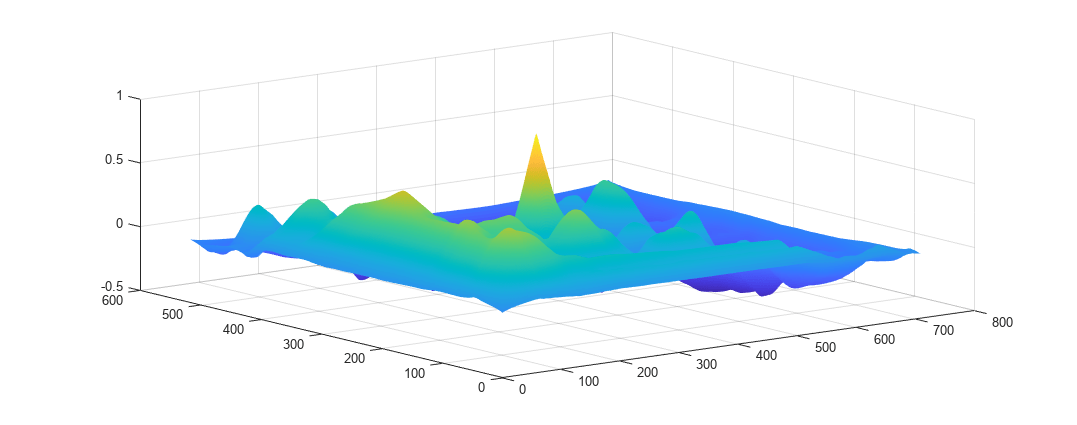
\includegraphics[width=0.9\textwidth]{images/normxcorr2_surface.png}
  \caption{Example of a surfaced produced by the normalised cross-correlation of a template with an image in MATLAB using the \texttt{normxcorr2} function \cite{mathworks_2023a}.}
  \label{fig:normxcorr2}
\end{figure}

\newpage
\subsection{Thresholding and Binarization}

Image thresholding, also known as binarization, is a process by which a threshold is applied to a grayscale image, producing a binary, black-and-white result \cite{mathworks_2023b}. Pixels with a grayscale value less than the threshold are represented by zero, and those larger than or equal to the threshold are represented by one \cite{opencv_2023b}.

The purpose of binarization is to remove background detail while enhacing details of importance. For example, Figure \ref{fig:imbinarize} presents the use of binarization to significantly enhance the readability of the words on a shadowed page.

\begin{figure}[ht]
  \centering
  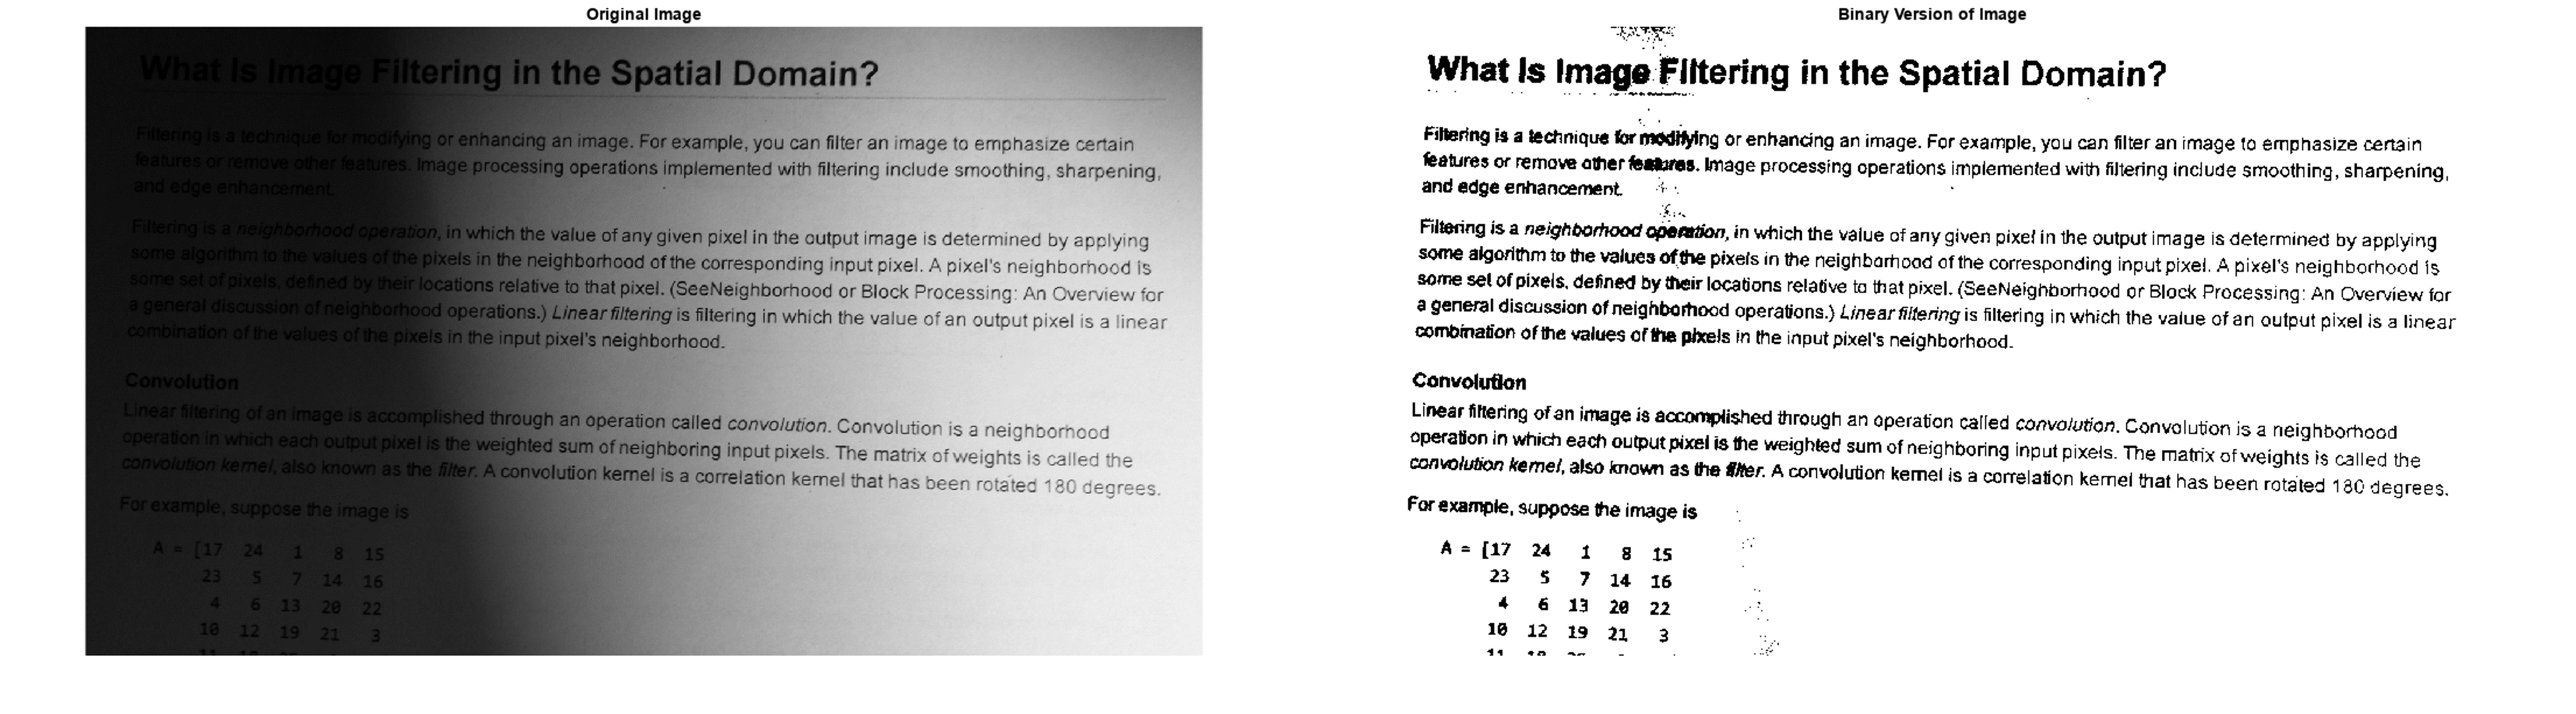
\includegraphics[width=\textwidth]{images/imbinarize_result.png}
  \caption{MATLAB function \texttt{imbinarize} used to enhance the text in an image \cite{mathworks_2023b}.}
  \label{fig:imbinarize}
\end{figure}

\newpage
\subsection{Hough Line Transform}

The Hough Transform is a technique that can be used to detect any shape in an image, as long as the shape can be represented in mathematical form \cite{opencv_2023c}. The Hough Line Transform (HLT), as the name suggests, detects lines in a binary image.

The HLT operates in polar coordinates, in which a line is defined by $\rho$ and $\theta$:
\begin{align}
  \rho = x \cos\theta + y \sin\theta
\end{align}
where $\theta$ defines an angle from the horizontal axis and $\rho$ defines the perpendicular distance from the line to the origin \cite{opencv_2023c}.

Suppose the HLT is performed on an image with one or more white lines against a black background. The algorithm defines an ``accumulator'' matrix with a cell for each possible combination of $\rho$ and $\theta$ \cite{opencv_2023c}. The size of this matrix depends on the desired resolution of $\rho$ and $\theta$, which are configurable parameters of the HLT algorithm \cite{opencv_2023c}.

For every white pixel in the image, the algorithm iterates through all possible angles $\theta$ and calculates a value for $\rho$ for each. For each $(\rho,\theta)$ pair, the corresponding cell in the accumulator is incremented by one \cite{opencv_2023c}. In this way, every white pixel on the line defined by $\rho$ and $\theta$ increments the respective cell in the accumulator. When the algorithm is finished, detected lines are identified in the accumulator as $(\rho,\theta)$ pairs with a value larger than some configurable threshold, representing lines with more than a certain number of colinear pixels \cite{opencv_2023c}.

The HLT is described as a ``transform'' because each white pixel is represented in the accumulator as a sinusoid, and the intersection of these sinusoids defines the detected lines. The representation of the image in the accumulator is known as the ``Hough space'' \cite{opencv_2023c}. Figure \ref{fig:hough_line} presents an example of lines in an image translated into the Hough space.

\begin{figure}[ht]
  \centering
  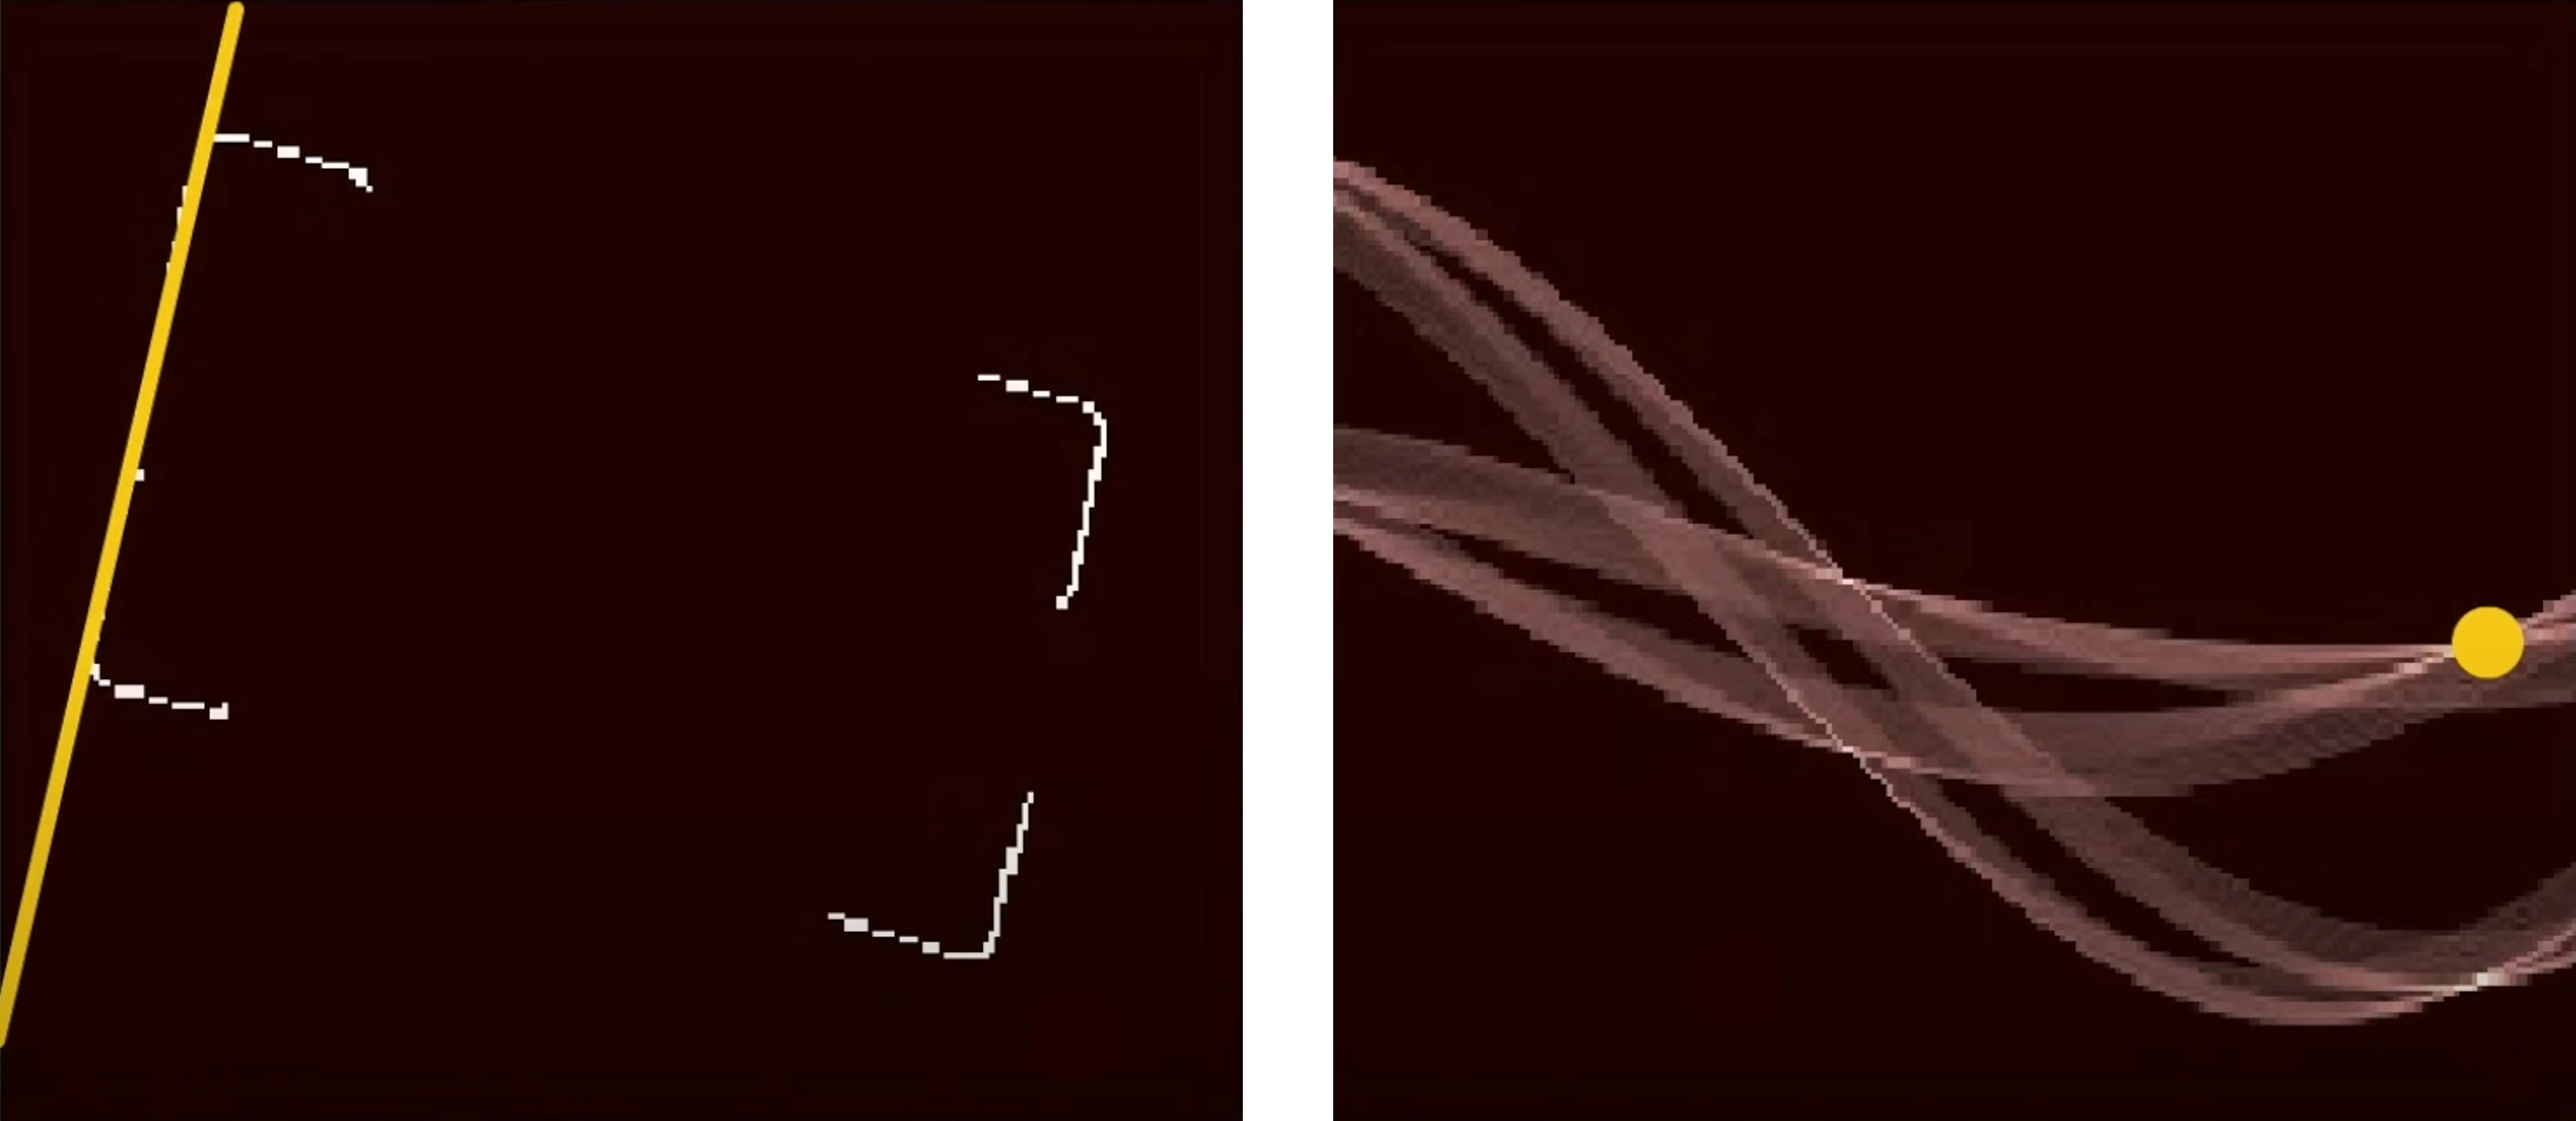
\includegraphics[width=0.8\textwidth]{images/hough_transform.png}
  \caption{Lines in an image represented in the Hough space; the yellow line on the left corresponds to the yellow point on the right \cite{korting_2016}.}
  \label{fig:hough_line}
\end{figure}

\newpage
\section{Methodology}

This section describes the procedure used to track the contact point between the pantograph and conducting cable in the pantograph video. Image analysis is performed on a frame-by-frame basis, thereby requiring the video first to be split into individual frames.

Two templates of the pantograph, A and B, are constructed from from frames 1 and 1300, respectively, by manually cropping the frames to isolate the pantograph. Template A represents the pantograph in a low position, and template B in a high position. Due to the position of the recording camera, the height of the pantograph affects the size of the template. By using two templates at different heights, the template matching consistently identifies the pantograph at all heights throughout the video.

After splitting the frames and creating the templates, the following steps are applied to each frame to identify the intersection point of the pantograph and the conducting cable.
\begin{enumerate}
  \item The frame is cropped to remove the black borders and watermark. This reduces the number of features in each frame, hence simplifying the image processing task.

  \item Template matching is performed on the frame using both templates A and B. The position reported by the better match is inferred to be the position of the pantograph.

  \item The frame is cropped to leave only the area directly above the pantograph, as determined by the position of the template match and the size of the matched template. Again, this reduces the features in the frame to simplify identifying the overhead cables.

  \item The frame is converted to HSV and the value channel is extracted. The frame consists of black cables against a light-coloured sky, so the value channel is useful for differentiating the cables from the background.

  \item The frame is binarized using an experimentally tuned threshold of 75. This effectively separates the overhead cables from the background.

  \item The Hough transform is applied to the binarized image with a $\rho$ resolution of 1 pixel, a $\theta$ resolution of 1 degree, and a threshold of 60\% of the height of the frame in pixels. The dynamic threshold scales approximately with the visible length of cable in the frame.

  \item The Hough transform outputs zero or more $(\rho,\theta)$ pairs. It can be observed that the conducting cable generally has a larger angle from the vertical than the suspension cable, so the $\theta$ angle is used to sort the detected lines.

  \item The sorted lines are checked in descending $\theta$ order, and the line with the largest angle between the expected range of angles is inferred to be the conducting cable. From observation, the expected range is up to $15^o$ on either side of the vertical. Constraining the angle reduces the likelihood of detecting cable support structures and other cables.

  \item The $\rho$ and $\theta$ values for the chosen line are used to construct a linear equation using:
  \begin{align}
    a = \cos\theta && b = \sin\theta && m = -\frac{a}{b} && c = \rho \left(b + \frac{a^2}{b}\right)
  \end{align}
  assuming $\theta \neq 0$. For cases where $\theta \approx 0$, the pantograph intersection is calculated directly using step 11.

  \item Given $m$ and $c$, the horizontal intersection of the line with the bottom of the frame is calculated by substituting $y=h$ into the standard equation of a line and solving for $x$:
  \begin{align}
    x = h - \frac{c}{m}
  \end{align}
  Since the frame is cropped directly above the pantograph, this approximates the intersection of the pantograph and conducting cable.

  \item For near vertical lines, $m$ and $c$ do not need to be calculated. Instead, the horizontal position of the intersect is simply $x=\rho$.

\end{enumerate}

\section{Results}

The detected horizontal position of the intersection between the pantograph and the conducting cable is plotted in Figure \ref{fig:results}.

\begin{figure}[ht]
  \centering
  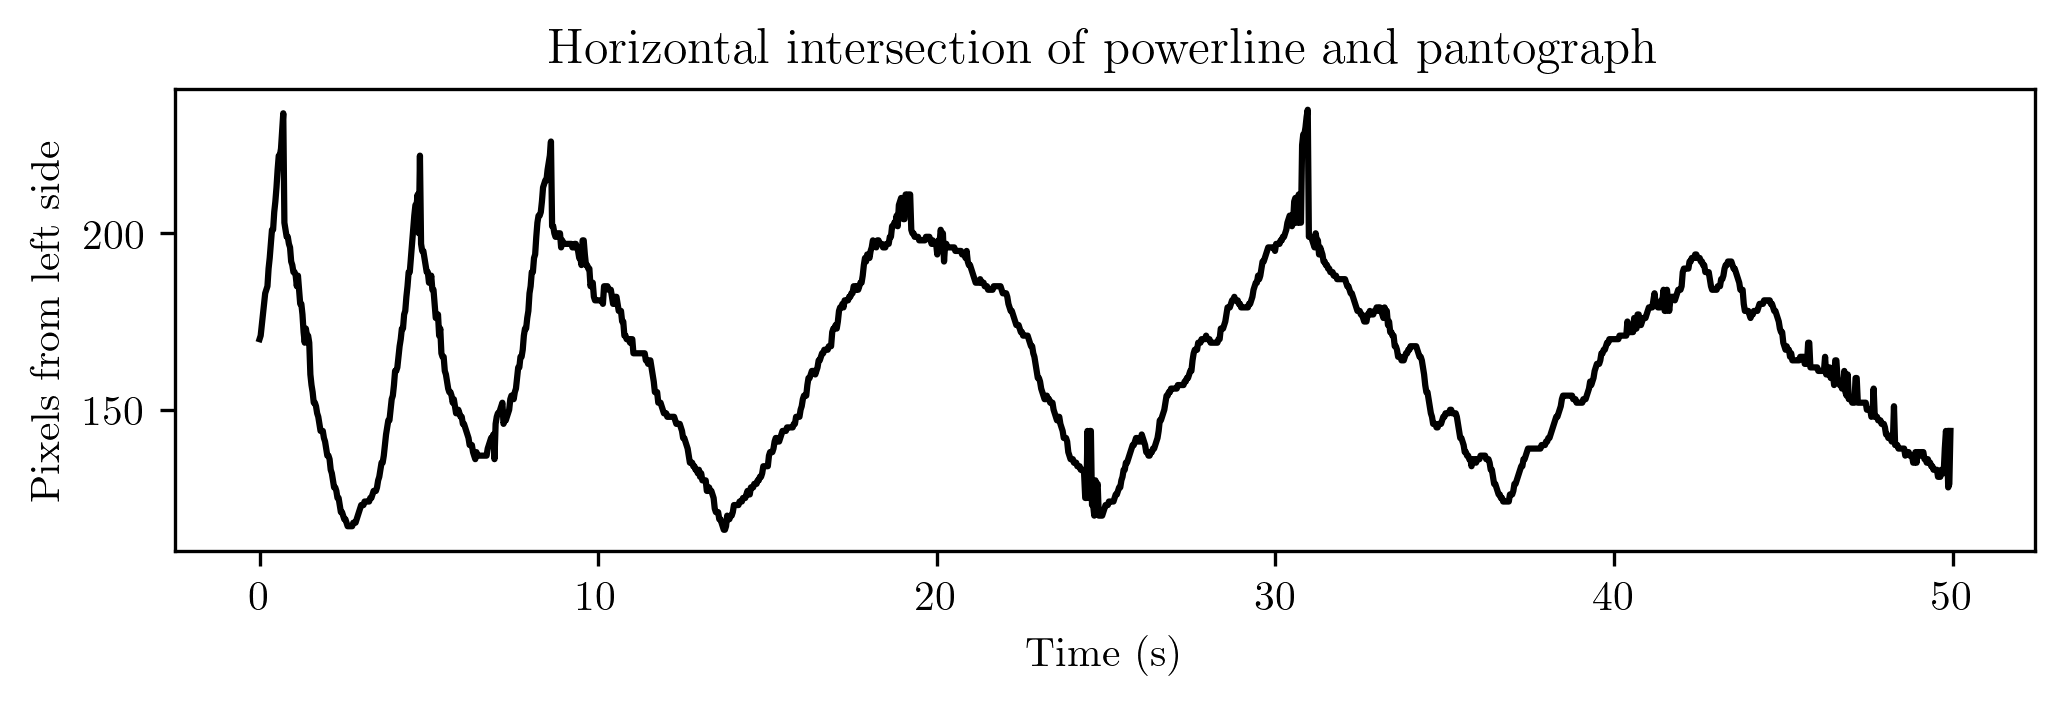
\includegraphics[width=0.8\textwidth]{images/intersection_position.png}
  \caption{Horizontal position of the conducting cable on the pantograph over time.}
  \label{fig:results}
\end{figure}

The results were additionally verified by drawing the intersection point on each frame and recombining the frames into a video. The solution is observed to track reasonbly well, though is often incorrect when the pantograph is near an overhead supporting structure.

\newpage
\section{Discussion}

This report has presented a method of detecting and tracking the contact point between a rail pantograph and conducting cable in a video. The conducting cable typically zig-zags horizontally across the top of the pantograph, and a similar pattern ought to be observed in the results.

Figure \ref{fig:results} demonstrates that the results corroborate the expectation. As mentioned in the previous section, the results can additionally be verified by drawing the intersection point in each frame.

It may be observed, however, that the plot becomes noisy in the second half. While some of the noise may be attributed to brief oscillatory motion of the conducting cable, much of the high frequency noise occurs when the solution misidentifies the conducting and suspension cables, and rapidly switches between the two. This occurs more frequently in the second half of the video because the cables remain much closer together.

Another notable feature of Figure \ref{fig:results} is the peak at approximately 25 seconds. This occurs when another conducting cable briefly passes over the pantograph. While Step 8 of the methodology succesfully filters out this cable for the majority of its overhead duration, there are nonetheless a few frames where the passing cable is misidentified as the conducting cable due to its larger angle from the vertical, resulting in a discrete jump in the results.

A final observation, also mentioned in the previous section, is that the detection is often incorrect in frames where the pantograph is near an overhead supporting structure. In these cases, the template matching often reports an incorrect pantograph position. This most likely occurs when the height of the pantograph is unequal to the height in either template. As a result, the size of the pantograph is slightly different to both templates, and parts of the supporting structure produce a better match than the pantograph.

One possible solution to all of the above issues is as follows. The range of possible positions of the intersection can be constrained by the fact that the motion of the cable is continuous (for high enough FPS). This knowledge can be used to eliminate large discrete jumps caused by misidentified cables or pantographs. However, depending on the implementation, this may be relatively computationally expensive for the benefit it offers.

Another possibility, though only for pantograph detection, is to use feature matching rather than template matching to find the pantograph. Feature matching is size and orientation invariant, making it more robust \cite{opencv_2023d}. However, this simultaneously makes it more challenging to implement and likewise may not be worth the additional computational complexity.

\section{Conclusion}

In summary, this report presents a largely successful solution to the problem of tracking the intersection of a rail pantograph and conducting cable in a video. The solution is observed to track reasonably well, except where the pantograph is near an overhead supporting structure. Reasons for noise and other imperfections in the results are discussed, and possible improvements are suggested.

%-----------------------
% Bibliography
%-----------------------
\newpage
\printbibliography[keyword={q2}]